\documentclass{article}
\usepackage[utf8]{inputenc}
\usepackage{amsmath, amssymb}
\usepackage{geometry}
\geometry{a4paper, margin=1in}
\usepackage{tikz}
\usetikzlibrary{cd, positioning}
\usepackage{booktabs}

\title{SpezSem Chapter 5 - Limits \& Colimits\\ \large Discussion Script and Content Outline}
\author{}
\date{}

\begin{document}

\maketitle

\section*{Introduction: Beyond the Abstract}
While Awodey provides a rigorous mathematical foundation using pullbacks, equalizers, and universal properties, our discussion will pivot to how these abstract concepts behave when we try to compute them, model physical systems with them, or scale them up in programming and database management.

% ---------------------------------------------------------
% PART 1: DATABASES
% ---------------------------------------------------------
\section{Part 1: The Database Approach}
While standard treatments of category theory focus heavily on abstract mathematical structures, applied category theory provides concrete, real-world models. One of the most intuitive applications of limits and colimits is found in the realm of databases.

\subsection{From Abstract Categories to Database Schemas}
In a standard mathematical depiction, a category $\mathcal{C}$ is defined by:
\begin{itemize}
    \item \textbf{Objects:} $A, B, C, \dots$
    \item \textbf{Arrows (Morphisms):} $f: A \to B$, $g: B \to C, \dots$
    \item \textbf{Composition:} $g \circ f: A \to C$
    \item \textbf{Identities:} $1_A: A \to A$
\end{itemize}

To understand how this models a database, we simply swap out the mathematical terminology for database terminology:
\begin{itemize}
    \item \textbf{Objects $\to$ Tables:} Specifically, the ID columns (or primary keys) of tables, as well as primitive data types (like Strings or Integers).
    \item \textbf{Arrows $\to$ Columns (Foreign Keys and Attributes):} An arrow $f: A \to B$ represents a non-ID column in table $A$ that references the ID column of table $B$ (an internal reference or foreign key), or a column in table $A$ that contains a primitive type like a String (an external reference).
    \item \textbf{Composition $\to$ Path Queries:} Following a foreign key from one table to another, and then another.
    \item \textbf{Category $\to$ Database Schema:} The directed graph of all tables and their relationships forms a finitely presented category $\mathcal{C}$.
\end{itemize}

\subsection{Visualizing the Category as Data}
To make this concrete, let's look at an example instance of a database with two interlocking tables: \texttt{Employee} and \texttt{Department}.

\vspace{0.5cm}
\begin{minipage}{0.55\textwidth}
    \centering
    \textbf{Employee Table} \\
    \vspace{0.2cm}
    \begin{tabular}{|l|l|l|l|}
    \hline
    \textbf{ID} & \textbf{FName} & \textbf{WorksIn} & \textbf{Mngr} \\ \hline
    1 & Alan & 101 & 2 \\ \hline
    2 & Ruth & 101 & 2 \\ \hline
    3 & Kris & 102 & 3 \\ \hline
    \end{tabular}
\end{minipage}
\begin{minipage}{0.4\textwidth}
    \centering
    \textbf{Department Table} \\
    \vspace{0.2cm}
    \begin{tabular}{|l|l|l|}
    \hline
    \textbf{ID} & \textbf{DName} & \textbf{Secr} \\ \hline
    101 & Sales & 1 \\ \hline
    102 & IT & 3 \\ \hline
    \end{tabular}
\end{minipage}
\vspace{0.5cm}

Here, the objects of our category are the ID columns (\texttt{Employee}, \texttt{Department}) and the type \texttt{String}. The arrows are the non-ID columns:
\begin{itemize}
    \item \texttt{WorksIn: Employee $\to$ Department} (Internal reference / foreign key)
    \item \texttt{FName: Employee $\to$ String} (External reference / attribute)
\end{itemize}

\textit{Visualization:} We can visualize this database schema as a directed graph:
\begin{center}
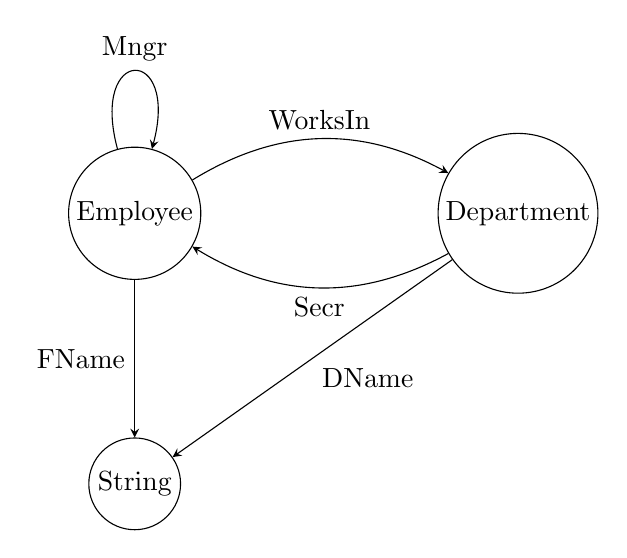
\begin{tikzpicture}[node distance=2cm and 3cm, auto, >={stealth}]
    \node[circle, draw, fill=white, text=black, inner sep=2pt] (E) {Employee};
    \node[circle, draw, fill=white, text=black, inner sep=2pt, right=of E] (D) {Department};
    \node[circle, draw, fill=white, inner sep=2pt, below=of E] (S) {String};
    
    \draw[->] (E) to[loop above] node {Mngr} (E);
    \draw[->] (E) to[bend left] node {WorksIn} (D);
    \draw[->] (D) to[bend left] node {Secr} (E);
    \draw[->] (E) to node[swap] {FName} (S);
    \draw[->] (D) to node {DName} (S);
\end{tikzpicture}
\end{center}

While the schema is the category itself, the actual data populating the tables at any given moment is represented as a set-valued functor $I: \mathcal{C} \to \mathbf{Set}$. Constraints are ensured by the fundamental rules of functors preserving composition.

\subsection{Data Migration and Inner Joins}
When organizations need to move data from an old database schema to a new one, they perform data migration. Category theory formalizes this automated reorganizing process using adjoint functors. 

If we have a functor $F: \mathcal{C} \to \mathcal{D}$ connecting two schemas, we can migrate data between them. The data migration functor $\Delta_F$ pulls back data along $F$. This functor always has two adjoints that perform powerful structural operations:
\begin{itemize}
    \item \textbf{Left Adjoint ($\Sigma_F$):} Sums or disjoint unions the data. It acts like a \texttt{UNION ALL} or a merge.
    \item \textbf{Right Adjoint ($\Pi_F$):} Pairs and queries data by taking products. In the terminology of database programmers, this structural pairing operation is what is commonly known as a \textbf{join} (or inner join). 
\end{itemize}

\subsection{Limits and Colimits in Queries}
The operations used to summarize, query, and manipulate database instances are explicitly driven by limits and colimits in the category of sets ($\mathbf{Set}$).

\textbf{1. The Classic Limit (Mathematical Representation)} \\
In a standard category, a limit for a diagram $D$ is a universal cone. If $X$ is the limit and $X'$ is any other cone over the diagram $D$, there is a unique arrow $k: X' \to X$ that makes the diagram commute for every object $D_i$ in $D$.

\begin{center}
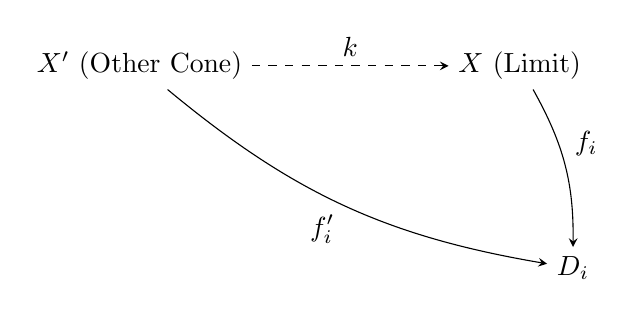
\begin{tikzpicture}[node distance=1.5cm and 2.5cm, auto, >={stealth}]
    \node (Xprime) {$X'$ (Other Cone)};
    \node (X) [right=of Xprime] {$X$ (Limit)};
    \node (Di) [below right=of Xprime, xshift=1.25cm, yshift=-0.5cm] {$D_i$};
    
    \draw[->, dashed] (Xprime) to node {$k$} (X);
    \draw[->, bend right=15] (Xprime) to node [swap] {$f'_i$} (Di);
    \draw[->, bend left=15] (X) to node {$f_i$} (Di);
\end{tikzpicture}
\end{center}

\textbf{2. The Query Interpretation (Inner Joins and Filters)} \\
When we apply this exact universal property to a database instance (a functor into $\mathbf{Set}$), the limit $X$ perfectly models a database query (like an inner join with a \texttt{WHERE} clause). A limit selects tuples that satisfy the equations or constraints of the schema.

\begin{itemize}
    \item \textbf{Diagram Objects ($D_i$):} The tables or data sets we want to query and join.
    \item \textbf{Limit Cone ($X$):} The \textbf{Result Set} of the query (the joined table). It selects tuples $(d_1, \dots, d_n)$ that perfectly match the morphisms of the schema, capturing the exact data satisfying the conditions.
    \item \textbf{Other Cone ($X'$):} Any arbitrary collection of candidate data.
    \item \textbf{Unique Arrow ($k$):} The canonical filter map. The universal property guarantees that the limit contains \textit{all} valid data satisfying the join constraints without any redundancy.
\end{itemize}

\begin{center}
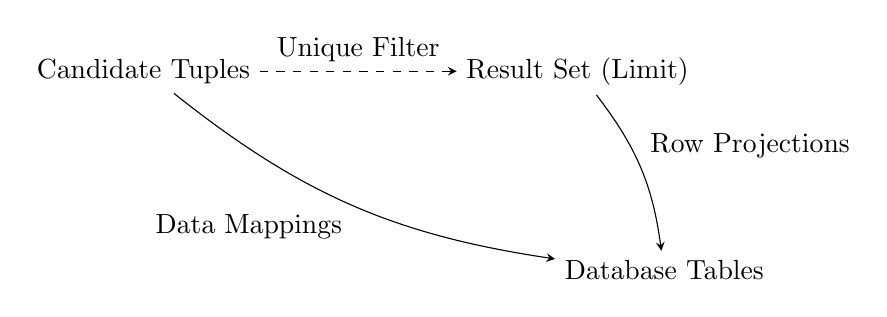
\begin{tikzpicture}[node distance=1.5cm and 2.5cm, auto, >={stealth}]
    \node (Xprime) {Candidate Tuples};
    \node (X) [right=of Xprime] {Result Set (Limit)};
    \node (Di) [below right=of Xprime, xshift=1.25cm, yshift=-0.5cm] {Database Tables};
    
    \draw[->, dashed] (Xprime) to node {Unique Filter} (X);
    \draw[->, bend right=15] (Xprime) to node [swap] {Data Mappings} (Di);
    \draw[->, bend left=15] (X) to node {Row Projections} (Di);
\end{tikzpicture}
\end{center}

% ---------------------------------------------------------
% PART 2: PROGRAMMING LANGUAGES
% ---------------------------------------------------------
\section{Part 2: The Programming Language Approach}
Category theory provides a meta-language for reasoning about computer programs at a declarative level. It encourages a global approach to problem solving, replacing imperative recipes with universal constructions.

\subsection{Declarative vs. Imperative Definitions}
In traditional programming, we build types imperatively. For instance, creating a Cartesian product is often described as a recipe: pick one element from one set, pick another element from another set, and assemble them into a pair. 

Category theory, however, defines a product \textit{declaratively} by specifying its universal properties. It asks: what is the best object that optimizes the property of factorizing the projections of other objects?

\subsection{Limits as Record Types (Products)}
The canonical implementation of a categorical product in a programming language is a pair, a struct in C, or a record type in Haskell. 

Consider a standard record type \texttt{PERSON} with two fields: \texttt{NAME} (a String) and \texttt{AGE} (an Integer). In category theory, this record type is exactly a product cone over a discrete graph with two nodes. 

\begin{center}
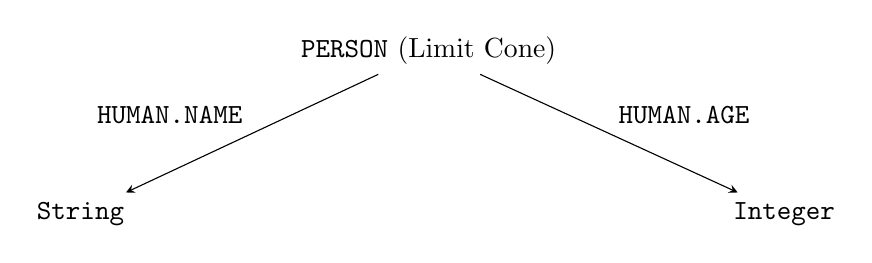
\begin{tikzpicture}[node distance=1.5cm and 2cm, auto, >={stealth}]
    \node (Person) {\texttt{PERSON} (Limit Cone)};
    \node (Name) [below left=of Person] {\texttt{String}};
    \node (Age) [below right=of Person] {\texttt{Integer}};
    
    \draw[->] (Person) to node [swap] {\texttt{HUMAN.NAME}} (Name);
    \draw[->] (Person) to node {\texttt{HUMAN.AGE}} (Age);
\end{tikzpicture}
\end{center}

In this categorical model, if \texttt{HUMAN} is a variable of type \texttt{PERSON}, the field selectors (\texttt{HUMAN.NAME} and \texttt{HUMAN.AGE}) act precisely as the coordinate projections of the limit cone. 

\subsection{Colimits as Variant Types (Sums)}
While limits model products and records, colimits model sum types, variants, and tagged unions. 

If \(A\) and \(B\) are data types, their sum \(A + B\) can be understood as the free variant or free union of those types. In a programming language, this requires canonical structure maps (or injections), such as \(i_1: A \to A + B\) and \(i_2: B \to A + B\). These injections act as type conversions, wrapping a specific type into the broader union type. 

The universal property of the coproduct tells us exactly how to write code that works with these types: for any functions \(f: A \to C\) and \(g: B \to C\), there is a unique function \([f, g]: A + B \to C\). In Haskell, this is \texttt{Either a b}; in Rust or C++, it is \texttt{Result} or \texttt{std::variant}. When we write a \texttt{switch} statement or a \texttt{match} expression, we are manually constructing this unique arrow \([f, g]\). By forcing us to handle both cases, colimits ensure our programs are \textbf{total} (no missing cases).

\textbf{Discussion Prompt:} \textit{"We saw that the pullback models constraints, and the colimit (sum) models choice. How does viewing types as limits/colimits (universal properties) change the way we design APIs? Is a `good' API one that exposes a universal property?"}

% ---------------------------------------------------------
% PART 3: LOGIC
% ---------------------------------------------------------
\section{Part 3: Propositions as Types}
One of the most beautiful and deep connections in category theory is the idea that propositions are types (and programs are proofs). This is often called the Curry-Howard correspondence. Under this view, limits and colimits take on a precise logical meaning: they map directly to the logical connectives AND and OR.

\subsection{Limits as Conjunction (AND)}
In logic, we think of a type \(A\) as a proposition, and a program or term of type \(A\) as a proof of \(A\). In this view, a \textbf{limit} corresponds to logical \textbf{conjunction}. 

\begin{itemize}
    \item \textbf{Product ($A \times B$):} The product of two propositions is their conjunction \(A \land B\). A proof of \(A \land B\) consists of a proof of \(A\) \textit{and} a proof of \(B\). 
    \item \textbf{Elimination Rule:} The projections \(\pi_1 : A \times B \to A\) and \(\pi_2 : A \times B \to B\) are exactly the logical rules for eliminating a conjunction. If you have a proof of "A AND B", you can extract a proof of "A".
    \item \textbf{Programming Example:} In code, this is the function \texttt{fst :: (a, b) -> a} or \texttt{fst(x, y) = x}. It extracts the first element of a pair.
    \item \textbf{Terminal Object (1):} The terminal object is the empty limit. It corresponds to the proposition \textit{True}. Every type has a unique map to it, meaning every proposition implies True.
\end{itemize}

\subsection{Colimits as Disjunction (OR)}
Dually, \textbf{colimits} correspond to logical \textbf{disjunction}.

\begin{itemize}
    \item \textbf{Coproduct ($A + B$):} The coproduct of two propositions is their disjunction \(A \lor B\). A proof of \(A \lor B\) is either a proof of \(A\) \textit{or} a proof of \(B\). 
    \item \textbf{Introduction Rule:} The injections \(\iota_1 : A \to A + B\) and \(\iota_2 : B \to A + B\) are the logical rules for introducing a disjunction. If you have a proof of "A", you can prove "A OR B".
    \item \textbf{Programming Example:} In Haskell, this is \texttt{Left :: a -> Either a b}. We are wrapping a value to satisfy the sum type.
    \item \textbf{Initial Object (0):} The initial object is the empty colimit. It corresponds to the proposition \textit{False}. From False, anything follows (\textit{ex falso quodlibet}), which is exactly the universal property of the initial object.
\end{itemize}

\subsection{Summary of the Logical Duality}
The duality between limits and colimits perfectly mirrors the duality between conjunction and disjunction.

\begin{center}
\begin{tabular}{@{}lll@{}}
\toprule
\textbf{Logic} & \textbf{Category Theory} & \textbf{Programming} \\
\midrule
True & Terminal Object (Limit) & \texttt{Unit} / \texttt{()} \\
False & Initial Object (Colimit) & \texttt{Void} \\
$A \land B$ (AND) & Product (Limit) & Record / Struct \\
$A \lor B$ (OR) & Coproduct (Colimit) & Variant / Sum Type \\
\bottomrule
\end{tabular}
\end{center}

\textbf{Discussion Prompt:} \textit{"If we think of a proof as a program, then proving a conjunction means producing a pair of values, and proving a disjunction means choosing one side and wrapping it. Given this deep correspondence, does designing a type system become a form of logical engineering?"}

% ---------------------------------------------------------
% PART 4: COMPUTATIONAL CATEGORY THEORY (BONUS)
% ---------------------------------------------------------
\section{Part 4: Bonus --- Computational Category Theory}
Because category theory is highly constructive, theorems that prove the existence of objects do so by explicit construction, meaning category theory can itself be viewed as a collection of algorithms. In Rydeheard and Burstall's \textit{Computational Category Theory}, constructive categorical proofs are translated directly into executable algorithms (written in Standard ML).

\subsection{Universal Properties as Computable Functions}
The authors bridge the gap between abstract math and code via a technique called \textit{Skolemization}. A universal mapping property (which mathematically asserts ``there exists a unique arrow...'') is represented computationally as a higher-order function. 
For example, a colimit is encoded as a data type containing two parts:
\begin{enumerate}
    \item The colimiting cocone itself (the apex object and its injection arrows).
    \item A function that accepts any other valid cocone as input and outputs the unique mediating arrow to it.
\end{enumerate}

\subsection{Algorithmic Construction of Colimits}
Instead of computing complex colimits from scratch, the authors construct an iterative algorithm based on the theorem that \textit{a category with an initial object, binary coproducts, and coequalizers has all finite colimits}. The algorithm recursively decomposes a finite diagram, computes the colimits of its sub-components using these three primitives, and stitches the results together.

This can be visualized as a generic factory function where the category acts as an API providing the three fundamental ``lego bricks'' (\texttt{initial\_object}, \texttt{coproduct}, and \texttt{coequalizer}):

\begin{verbatim}
def compute_finite_colimit(diagram, category):
    # BASE CASE: No edges. Use Bricks 1 & 2 (Initial Object & Coproduct)
    if diagram.edges.is_empty():
        colimit = category.initial_object()
        for obj in diagram.objects:
            colimit = category.coproduct(colimit, obj)
        return colimit

    # RECURSIVE CASE: Edges exist. Use Brick 3 (Coequalizer)
    else:
        single_edge = diagram.edges.pop()
        partial_colimit = compute_finite_colimit(diagram, category)
        return category.coequalizer(partial_colimit, single_edge)
\end{verbatim}

\subsection{Limits via Duality}
The authors leverage the strict duality of category theory to halve their codebase. Rather than writing a separate recursive algorithm to compute finite limits, they implement a \texttt{dual\_colimit} function. To compute a limit, the program:
\begin{itemize}
    \item Reverses the arrows of the input diagram to form a diagram in the opposite category.
    \item Runs the existing colimit algorithm on this dual diagram.
    \item Reverses the arrows of the resulting colimiting cocone to yield the limiting cone in the original category.
\end{itemize}

\subsection{Application: Unification as a Coequalizer}
A major computational application presented in the book is \textit{term unification}---a core algorithm in automated theorem proving, type inference, and logic programming (e.g., Prolog). The authors demonstrate that finding the most general unifier (MGU) for a system of equations is mathematically equivalent to computing a \textbf{coequalizer} in the category of terms and substitutions.

\end{document}